\documentclass[11pt]{article}
\usepackage[utf8]{inputenc}
\usepackage[T1]{fontenc}
\usepackage{amsmath,amssymb}
\usepackage{geometry}
\usepackage{listings}
\usepackage{xcolor}
\usepackage{hyperref}
\usepackage{tikz}
\usepackage{booktabs}
\usepackage{enumitem}
\usetikzlibrary{calc, arrows.meta, positioning, fit, shapes.geometric}

\geometry{margin=2.2cm}

\lstdefinelanguage{Rust}{
  keywords={fn,let,mut,for,in,if,else,while,loop,match,return,struct,impl,pub,use,mod,as,where,move,ref,self,Self,crate,super,async,await,unsafe,const,static,type,enum,trait,dyn,true,false,continue,break},
  keywordstyle=\color{blue!70!black}\bfseries,
  ndkeywords={Vec,Vec3,Mat4,Mesh,MeshVertex,SceneNode,Scene,Tree,Shape,PbrMaterial,RenderState,FrameCtx,EngvisApp,Aabb,SubMesh,MeshTopology,u32,usize,f32,f64,bool,Option,Some,None,Result,Ok,Err,String,PathBuf,Path},
  ndkeywordstyle=\color{purple!70!black}\bfseries,
  sensitive=true,
  comment=[l]{//},
  morecomment=[s]{/*}{*/},
  commentstyle=\color{green!50!black}\itshape,
  stringstyle=\color{red!70!black},
  morestring=[b]",
}

\lstset{
  basicstyle=\ttfamily\footnotesize,
  breaklines=true,
  frame=single,
  language=Rust,
  showstringspaces=false,
  tabsize=2,
}

\title{The \texttt{engvis} UI Shell:\\
       Menu Bar, Workflow Panels, Status Bar,\\
       and Mesh I/O for Implicit Surface Visualization}
\author{engvis}
\date{\today}

\begin{document}
\maketitle

\begin{abstract}
This note documents the user-interface layer that wraps the
\texttt{engvis} implicit surface viewer.  Three things are described:
the four-region \texttt{egui} layout (top menu, left numbered workflow,
right detail panel, bottom status bar); a small triangle-mesh I/O layer
covering OBJ\,/\,STL\,/\,PLY (built on \texttt{tobj}, \texttt{stl\_io}
and \texttt{ply-rs-bw}); and an extended catalogue of built-in implicit
surfaces --- sphere, torus, gyroid, Schwarz P, Schwarz D, Schoen IWP,
Neovius --- together with arbitrary user-typed expressions parsed via
\texttt{fidget-rhai}.  The accompanying source files are
\texttt{src/main.rs} and \texttt{src/mesh\_io.rs}.
\end{abstract}

% =====================================================================
\section{Goals and Scope}

The viewer must let a user, without leaving the window:
\begin{enumerate}[leftmargin=2em]
  \item pick or type an implicit expression $f(x,y,z)$,
  \item polygonise it with one of two backends
        (Marching Cubes 33 or Manifold Dual Contouring),
  \item adjust the display (surface, points, edges, opacity, overlays),
  \item read off topology metrics
        $V,E,F,\chi=V-E+F$ and watertightness,
  \item import and export triangle meshes in OBJ, STL, PLY
        (and load glTF for textured scenes).
\end{enumerate}

The principle followed throughout is \emph{do not reinvent}:
all parsing, dialog and IO work is delegated to mature crates
(Table~\ref{tab:crates}).

\begin{table}[h]
\centering
\caption{External crates used by the UI layer.}
\label{tab:crates}
\begin{tabular}{lll}
\toprule
\textbf{Concern} & \textbf{Crate} & \textbf{Role} \\ \midrule
Immediate-mode GUI    & \texttt{egui 0.33}     & widgets and layout \\
File dialog           & \texttt{rfd 0.15}      & native open/save \\
OBJ reader            & \texttt{tobj 4.0}      & mesh import \\
STL read+write        & \texttt{stl\_io 0.8}   & binary STL IO \\
PLY reader            & \texttt{ply-rs-bw 2.0} & ASCII / LE / BE \\
Expression $\to$ Tree & \texttt{fidget-rhai 0.4.3} & string $\to$ \lstinline|Tree| \\
Topology              & \texttt{engvis-core}   & $V,E,F,\chi$ \\
\bottomrule
\end{tabular}
\end{table}

% =====================================================================
\section{Window Layout}

The window is partitioned into four \texttt{egui} panels plus a central
3D viewport, as shown in Figure~\ref{fig:layout}.

\begin{figure}[h]
\centering
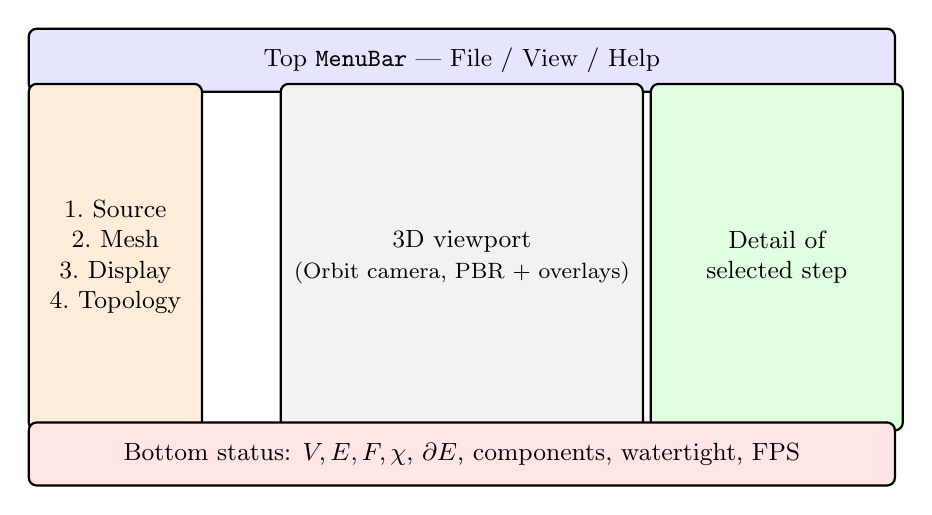
\begin{tikzpicture}[
    every node/.style={font=\small},
    panel/.style={draw, thick, minimum height=8mm, minimum width=20mm,
                  rounded corners=1mm, align=center},
]
  \node[panel, minimum width=110mm, fill=blue!10] (top)
        at (0,3.0) {Top \texttt{MenuBar} --- File / View / Help};
  \node[panel, minimum width=22mm, minimum height=44mm, fill=orange!15]
        (left) at (-4.4, 0.5) {1.~Source\\2.~Mesh\\3.~Display\\4.~Topology};
  \node[panel, minimum width=46mm, minimum height=44mm, fill=gray!10]
        (center) at (0, 0.5) {3D viewport\\\footnotesize(Orbit camera, PBR + overlays)};
  \node[panel, minimum width=32mm, minimum height=44mm, fill=green!12]
        (right) at (4.0, 0.5) {Detail of\\selected step};
  \node[panel, minimum width=110mm, fill=red!10] (bot)
        at (0,-2.0) {Bottom status: $V,E,F,\chi$, $\partial E$, components, watertight, FPS};
\end{tikzpicture}
\caption{Four-panel egui layout.  The left panel is the contract
(``what to do'', numbered); the right panel is the implementation
(``how'').  Status bar reflects the topology of the currently shown mesh.}
\label{fig:layout}
\end{figure}

\subsection{Top menu bar}

Constructed with \texttt{egui::TopBottomPanel::top} and the new 0.33
\texttt{MenuBar} container.  Three top-level menus:
\begin{description}[style=nextline]
  \item[File] \emph{Open mesh\ldots} (OBJ\,/\,STL\,/\,PLY\,/\,glTF),
              \emph{Save current mesh as \{OBJ,STL,PLY\}\ldots},
              \emph{Quit}.
              File pickers are native via \texttt{rfd::FileDialog};
              the picked path is written to
              \lstinline|App::pending_load| /
              \lstinline|App::pending_save| and serviced at the
              start of the next \lstinline|ui()| call so that file
              I/O never happens inside an open menu.
  \item[View] toggles for surface, grid, point overlay, bounding
              wireframe, MS boundary loops.
  \item[Help] one-line description and the custom-expression syntax.
\end{description}

\subsection{Left workflow panel (numbered, trait-style)}

A simple \lstinline|enum Step { Source, Mesh, Display, Topology }|
governs which detail page the right panel renders.
The numbered labels are rendered as \texttt{ui.selectable\_label}s so
that the panel acts like a four-row tab strip.

\subsection{Right detail panel}

A \texttt{match} on \lstinline|self.current_step| dispatches to one of
four small UI methods.  Each method writes back into \lstinline|App|
fields and sets \lstinline|self.needs_remesh = true| when it changes
something that requires re-polygonisation.

\subsection{Bottom status bar}

A horizontal strip showing the topology of the most recent build:
\[
  V,\ E,\ F,\ \chi = V-E+F,\ \#\partial E,\
  \text{\#components},\ \text{watertight}.
\]
This information is produced by
\lstinline|engvis_core::topology::compute_topology| (an existing
half-edge analyser) and cached in
\lstinline|App::last_topology|.

\subsection{Per-frame data flow}

Figure~\ref{fig:frame} shows the order of operations inside
\lstinline|App::ui|.

\begin{figure}[h]
\centering
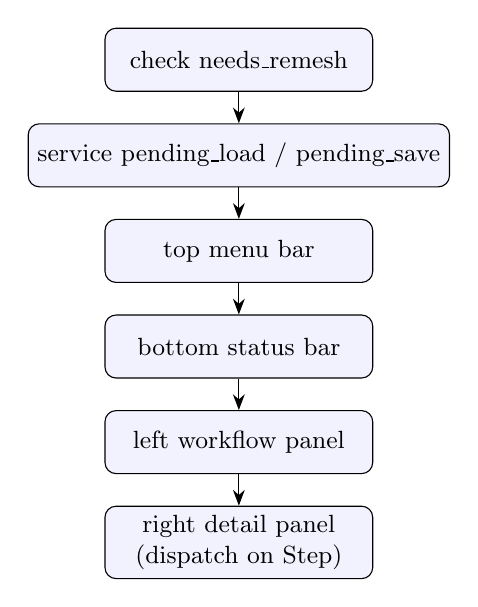
\begin{tikzpicture}[
    >={Stealth[length=2mm]},
    every node/.style={font=\small},
    box/.style={draw, rounded corners, minimum height=8mm,
                minimum width=34mm, align=center, fill=blue!5},
    dec/.style={draw, diamond, aspect=2.2, fill=yellow!15, align=center,
                inner sep=0.8mm},
]
  \node[box] (a) {check \lstinline|needs_remesh|};
  \node[box, below=4mm of a] (b) {service \lstinline|pending_load| /
                                  \lstinline|pending_save|};
  \node[box, below=4mm of b] (c) {top menu bar};
  \node[box, below=4mm of c] (d) {bottom status bar};
  \node[box, below=4mm of d] (e) {left workflow panel};
  \node[box, below=4mm of e] (f) {right detail panel\\(dispatch on \lstinline|Step|)};
  \draw[->] (a)--(b);
  \draw[->] (b)--(c);
  \draw[->] (c)--(d);
  \draw[->] (d)--(e);
  \draw[->] (e)--(f);
\end{tikzpicture}
\caption{Per-frame UI sequence inside \lstinline|App::ui|.  Pending
file actions are absorbed at the top so that a mesh swap is reflected
in every panel below in the same frame.}
\label{fig:frame}
\end{figure}

% =====================================================================
\section{Implicit Surface Library}

Each built-in surface is a function returning a Fidget
\lstinline|Tree|.  Trees are then handed to either Dual Contouring
(\texttt{fidget-mesh}) or our Marching Cubes 33 implementation.

\subsection{Closed-form definitions}

Let $(x,y,z)\in\mathbb{R}^3$, $k>0$ a period scale.  We polygonise
$\{f=0\}$ on $\Omega=[-1,1]^3$.

\begin{align}
  \text{Sphere} \quad &
    \sqrt{x^2+y^2+z^2} - 0.8 = 0
    \\[2pt]
  \text{Torus} \quad &
    \bigl(\sqrt{x^2+y^2}-R\bigr)^2 + z^2 - r^2 = 0,
    \ R{=}0.6,\ r{=}0.2
    \\[2pt]
  \text{Gyroid} \quad &
    \sin(kx)\cos(ky) + \sin(ky)\cos(kz) + \sin(kz)\cos(kx) = 0
    \\[2pt]
  \text{Schwarz P} \quad &
    \cos(kx)+\cos(ky)+\cos(kz) = 0
    \\[2pt]
  \text{Schwarz D} \quad &
    \begin{aligned}[t]
    & \sin(kx)\sin(ky)\sin(kz) + \sin(kx)\cos(ky)\cos(kz) \\
    +\,& \cos(kx)\sin(ky)\cos(kz) + \cos(kx)\cos(ky)\sin(kz) = 0
    \end{aligned}
    \\[2pt]
  \text{Schoen IWP} \quad &
    2\bigl[\cos(kx)\cos(ky)+\cos(ky)\cos(kz)+\cos(kz)\cos(kx)\bigr] \nonumber\\
    &\quad - \bigl[\cos(2kx)+\cos(2ky)+\cos(2kz)\bigr] = 0
    \\[2pt]
  \text{Neovius} \quad &
    3\bigl[\cos(kx)+\cos(ky)+\cos(kz)\bigr]
    + 4\cos(kx)\cos(ky)\cos(kz) = 0
\end{align}

\noindent
The Triply-Periodic Minimal Surfaces (TPMS) all use $k=3$.  The gyroid
uses $k=4$ to fit a few periods inside $\Omega$.  The variant
\textit{gyroid-sphere} reuses the gyroid expression and clips the
resulting open patch to the unit ball post-mesh --- see the existing
\texttt{gyroid-sphere-clip} document.

\subsection{User-typed expressions via \texttt{fidget-rhai}}

\texttt{fidget-rhai::engine()} returns a Rhai engine pre-loaded with:
\begin{itemize}[leftmargin=2em]
  \item \texttt{x, y, z} as \lstinline|Tree| primitives (not numbers);
  \item all elementary operators (\verb|+ - * / |) overloaded to build
        new \lstinline|Tree| nodes rather than evaluate;
  \item \texttt{sin, cos, sqrt, abs, exp, log,} $\ldots$ as
        tree-producing free functions.
\end{itemize}
The user types e.g.
\begin{center}\lstinline|sin(4*x)*cos(4*y) + sin(4*y)*cos(4*z) + sin(4*z)*cos(4*x)|\end{center}
into the right-panel \texttt{TextEdit::multiline} widget.  We then
call:
\begin{lstlisting}
let engine = fidget_rhai::engine();
let tree: fidget_core::context::Tree = engine.eval(src)?;
\end{lstlisting}
On error the message is shown in red below the editor and the surface
build is skipped (the status bar shows ``build failed'').

% =====================================================================
\section{Mesh I/O Layer (\texttt{src/mesh\_io.rs})}

\subsection{Format dispatch}

\lstinline|MeshFormat::from_path| inspects the file extension and the
two top-level functions \lstinline|load_mesh| / \lstinline|save_mesh|
dispatch (Figure~\ref{fig:io}).

\begin{figure}[h]
\centering
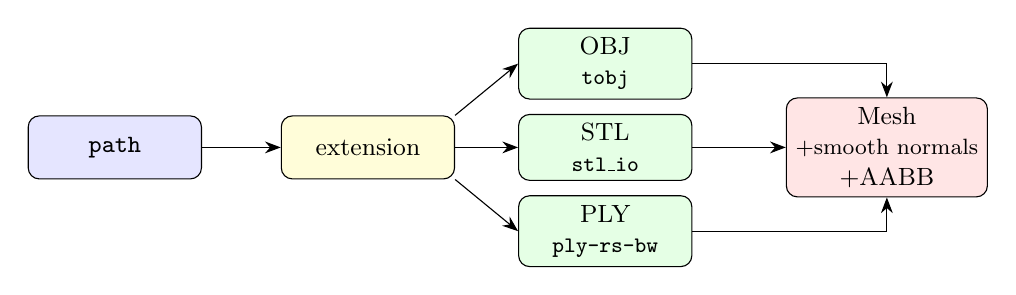
\begin{tikzpicture}[
    >={Stealth[length=2mm]},
    every node/.style={font=\small},
    box/.style={draw, rounded corners, minimum height=8mm,
                minimum width=22mm, align=center},
]
  \node[box, fill=blue!10]   (root) {\texttt{path}};
  \node[box, fill=yellow!15] (disp) [right=of root] {extension};
  \node[box, fill=green!10]  (obj)  [above right=2mm and 8mm of disp]
        {OBJ\\\footnotesize \texttt{tobj}};
  \node[box, fill=green!10]  (stl)  [right=8mm of disp]
        {STL\\\footnotesize \texttt{stl\_io}};
  \node[box, fill=green!10]  (ply)  [below right=2mm and 8mm of disp]
        {PLY\\\footnotesize \texttt{ply-rs-bw}};
  \node[box, fill=red!10]    (mesh) [right=42mm of disp]
        {\lstinline|Mesh|\\\footnotesize +smooth normals\\+AABB};
  \draw[->] (root)--(disp);
  \draw[->] (disp.north east)--(obj.west);
  \draw[->] (disp)--(stl);
  \draw[->] (disp.south east)--(ply.west);
  \draw[->] (obj.east)  -| (mesh.north);
  \draw[->] (stl.east)  -- (mesh.west);
  \draw[->] (ply.east)  -| (mesh.south);
\end{tikzpicture}
\caption{Format dispatch in \texttt{mesh\_io}.  Whatever the source,
positions and indices are normalised and a single helper computes
area-weighted vertex normals plus an AABB.}
\label{fig:io}
\end{figure}

\subsection{Smooth-normal helper}

Imported meshes typically carry no normals (STL stores per-face
normals only; OBJ frequently omits \texttt{vn}).  We compute
area-weighted vertex normals once during construction:
\[
  \mathbf{n}_v = \mathrm{normalize}\!\!\sum_{T\ni v}\!
                 (\mathbf{p}_1-\mathbf{p}_0)\times(\mathbf{p}_2-\mathbf{p}_0).
\]

\subsection{Writers}

\begin{itemize}[leftmargin=2em]
  \item \textbf{OBJ}: a $\sim 20$-line writer emitting
        \texttt{v / vn / f a//a b//b c//c}.  No external writer crate
        is needed; the format is trivially small.
  \item \textbf{STL}: \lstinline|stl_io::write_stl| with a freshly
        recomputed face normal per triangle.
  \item \textbf{PLY}: a $\sim 20$-line ASCII PLY writer.  The
        typed-element API of \texttt{ply-rs-bw} is overkill for a
        one-shot export.
\end{itemize}

% =====================================================================
\section{State Diagram of \texttt{App}}

The user-visible state of the app is captured by a handful of fields;
Figure~\ref{fig:states} shows the transitions that trigger a remesh.

\begin{figure}[h]
\centering
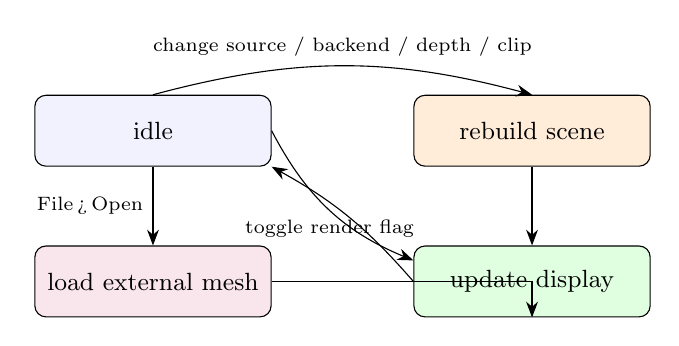
\begin{tikzpicture}[
    >={Stealth[length=2mm]},
    every node/.style={font=\small},
    state/.style={draw, rounded corners, minimum height=9mm,
                  minimum width=30mm, align=center, fill=blue!5},
]
  \node[state] (idle) {idle};
  \node[state, right=18mm of idle, fill=orange!15] (rebuild) {rebuild scene};
  \node[state, below=10mm of rebuild, fill=green!12] (display) {update display};
  \node[state, below=10mm of idle, fill=purple!10]  (load) {load external mesh};
  \draw[->] (idle.north) to[bend left=15]
        node[above, midway, font=\scriptsize]{change source / backend / depth / clip}
        (rebuild.north);
  \draw[->] (rebuild) -- (display);
  \draw[->] (idle.east) to[bend right=20]
        node[below, midway, font=\scriptsize]{toggle render flag} (display);
  \draw[->] (display.west) to[bend right=10] (idle.south east);
  \draw[->] (idle) -- node[left, font=\scriptsize]{File\,>\,Open} (load);
  \draw[->] (load.east) -| (display.south);
\end{tikzpicture}
\caption{Coarse state diagram.  Source, backend, depth, MS-loops and
clip toggles all flip \lstinline|needs_remesh|; pure display toggles
(grid, points, opacity, edge color) update the next frame without a
remesh.}
\label{fig:states}
\end{figure}

% =====================================================================
\section{Build Notes}

\paragraph{Dependency conflict.}
At the time of writing, \texttt{facet-path 0.44.5} declares an upstream
dependency on \texttt{facet-core "\^{}0.45"} while sibling crates in
the \texttt{fidget} stack still pin \texttt{facet 0.44.x}, which itself
uses \texttt{facet-core 0.44.x}.  This produces a duplicate
\texttt{facet-core} in the dependency graph and the trait
\lstinline|Facet<'_>| ceases to be implemented for \lstinline|Tree|.
We pin via
\begin{lstlisting}[language=bash]
cargo update -p facet-path --precise 0.44.4
\end{lstlisting}
This is recorded in \texttt{Cargo.lock}; no source code change is
needed.

\paragraph{Verification.}
\begin{lstlisting}[language=bash]
cargo build -p engvis        # clean build, no warnings from this crate
cargo run   -p engvis        # window opens; default surface gyroid-sphere
\end{lstlisting}
Status-bar readouts are produced by
\lstinline|compute_topology| immediately after each successful mesh
build, ensuring the displayed $V,E,F,\chi$ correspond to exactly the
geometry on screen.

\end{document}
